\section{Sphinx}\label{sec:sphinx}

Sphinx packets consist of a header and an encrypted payload. 
The header itself contains a \textit{cryptographic element $\alpha$} (e.g. $g^x$ or an elliptic curve point), \textit{encrypted routing information $\beta$}, and an \textit{integrity tag $\gamma$}, as illustrated in Figure \ref{fig:sphinx_structure}.

\begin{figure}[h]
    \centering
    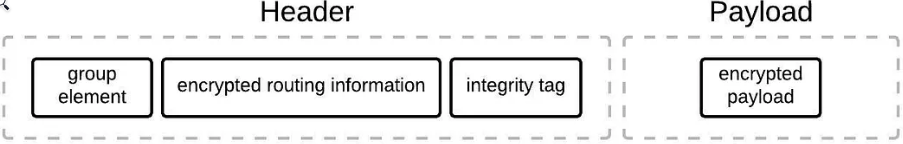
\includegraphics[width=0.9\linewidth]{Images/sphinx_structure.png}
    \caption{Structure of sphinx packet. \href{https://blog.nymtech.net/sphinx-tl-dr-the-data-packet-that-can-anonymize-bitcoin-and-the-internet-18d152c6e4dc}{[source]}}
    \label{fig:sphinx_structure}
\end{figure}

The \textit{encrypted routing information ($\beta$)} is constructed in layers, applied in reverse order along the path.
First, the final destination is encrypted, and an integrity tag ($\gamma_i$) is computed. 
The IP address of the last mixnode ($n_i$) is then prepended.
As shown by Figure \ref{fig:sphinx_header}, this process repeats iteratively: each new header is encrypted, an integrity tag ($\gamma_{i-1}$) is computed, and the IP address of the preceding mixnode ($n_{i-1}$) is prepended.
This layered encryption ensures that each mixnode can only decrypt its own layer, revealing the next forwarding address while preserving end-to-end confidentiality and protecting against tampering.

\begin{figure}[h]
    \centering
    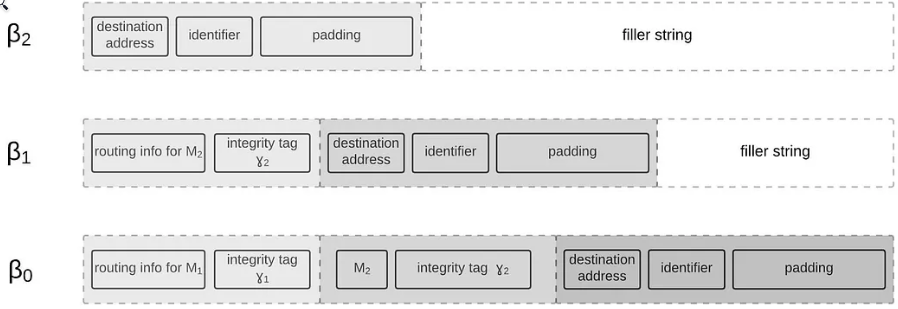
\includegraphics[width=\linewidth]{Images/sphinx_header.png}
    \caption{Sphinx encrypted routing information encapsulation. \href{https://blog.nymtech.net/sphinx-tl-dr-the-data-packet-that-can-anonymize-bitcoin-and-the-internet-18d152c6e4dc}{[source]}}
    \label{fig:sphinx_header}
\end{figure}

To encrypt the routing information, the nym client\todo{previously "user" but JT prefers "nym client"} first chooses a nonce $x$ and compute $\alpha = g^x$ as the \textit{cryptographic element} of the header.
Since each mixnode $i$ has a private key $x_i$ and a public key $y_i = g^{x_i}$, the user can create a shared secret $s_i$ with mixnode $i$ as followed: $s_i = y_i^x = (g^{x_i})^x$. 
Then the mixnode $i$ receiving the packet will get $\alpha$ allowing him to compute the shared secret as followed: $s_i = \alpha^{x_i} = (g^x)^{x_i}$.

Instead of sending a unique \textit{cryptographic element $\alpha$} at each node in the path, the sphinx format uses a single \textit{cryptographic element $\alpha$}, which is progressively modified at each node. 
Each mixnode updates the cryptographic element using its shared secret as follows:  
$$\alpha_{i+1} = \alpha_i^{\text{hash}(\alpha_i, s_i)}$$
Thus, the user iteratively computes the shared secrets in the path's order as: 
$$
\begin{aligned}
    \alpha_0 &= g^{x}, & s_0 &= y_{n_0}^{x}, & b_0 &= \text{hash}(\alpha_0, s_0) \\
    \alpha_1 &= g^{x b_0}, & s_1 &= y_{n_1}^{x b_0}, & b_1 &= \text{hash}(\alpha_1, s_1) \\
    &\vdots & &\vdots & &\vdots \\
    \alpha_i &= g^{x b_0 \cdots b_{i-1}}, & s_i &= y_{n_i}^{x b_0 \cdots b_{i-1}}, & b_i &= \text{hash}(\alpha_i, s_i)
\end{aligned}
$$
This formulation ensures that each mixnode can independently derive the necessary cryptographic elements without requiring the full path’s information, preserving privacy and unlinkability.  
\newline

The \textit{encrypted routing information ($\beta$)} is computed, as illustrated in Figure\todo{$\sim$\textbackslash ref\{\}} \ref{fig:sphinx_header}, by processing the path in reverse order. 
This involves XORing the routing information ($\beta_{i-1}$) from the previous layer (with the node's address and integrity tag) with a value derived from the shared secret $s_i$. 
Then prepending this new encrypted routing information ($\beta_i$) with an integrity tag ($\gamma_i$) and the previous mixnode address (remember we build it in reverse order).
We repeat the same process for each layer (i.e. each mixnode in the path).

\begin{figure}[H]
    \centering
    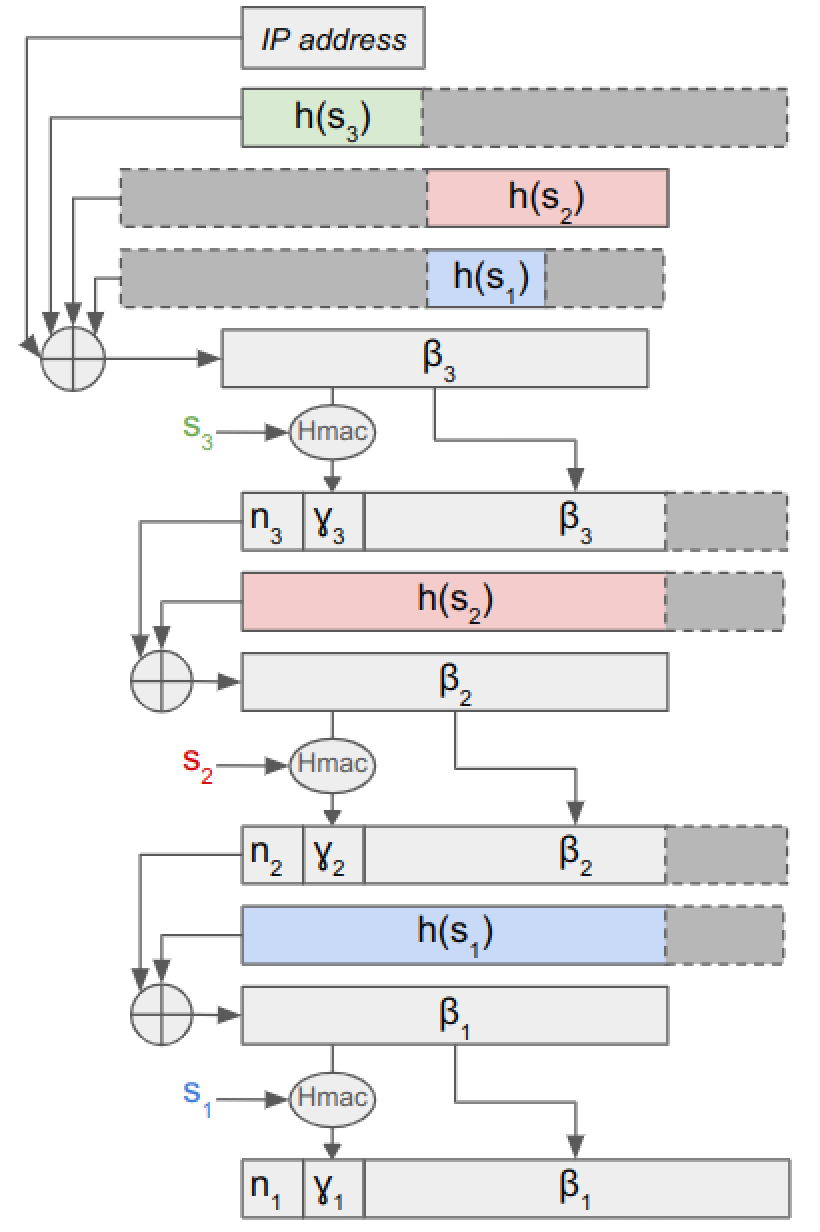
\includegraphics[width=0.5\linewidth]{Images/header_cipher.png}
    \caption{Construction of the Sphinx header (modified from \cite{sphinx}) [TO FIX: $h(s_1)$ at first XOR]}
    \label{fig:header_cipher}
\end{figure}
\todo[inline]{JT: Explain what the modifications are}
\todo[inline]{JT: Might help to put some (1) (2) (3) labels into the figure and refer to these labels in the text.}

% first round
The first round of XOR operations differs from the others because it requires combining parts of all shared secrets. 
Specifically, the destination address is XORed with the last node’s shared secret, truncated to match the address size.
Next, the result is concatenated with the XORed values of the ending parts of the shared secrets from the other nodes in the path. 
This ensures that when the entire header is XORed with the full shared secret, these appended values cancel out, allowing the header to be processed in reverse order by the mixnodes.
This design choice guarantees fixed-size headers, enabling fixed-size packets which is a crucial property in mixnets for maintaining unlinkability.

\todo[inline]{JT: Now maybe follow up with an example of the attack from the introduction?
We should also compare computational overheads from attack vs. the new protocol design.}



\section{Multi-Party Computation (MPC)}

The first approach to ensuring trust in the Sphinx header is to prevent user manipulation by decentralizing the header construction to Trusted Third Parties (TTP) through the use of Multi-Party Computaftion (MPC).

We consider TTPs as \textit{honest-but-curious}.\tothink{What if malicous TTP...}
This means that they follow the protocol correctly but may attempt to infer additional information from the data they process.
Our design aims to ensure that TTPs must not be able to infer any information about the shared secrets $s_i$ nor the mixnodes involved in the path, even when TTP are colliding (assuming that at least one TTP remains honest).
\todo{JT: In the Nym ecosystem, who are the TTPs, who operates them, what exactly are they trusted for?}
\newline


% Overall path selection:
% 1) Users choose the path
% 2) TTP randomly choose the path (without knowing it)

% Overall schema 
% 1̶)̶ ̶O̶n̶e̶ ̶T̶T̶P̶ ̶p̶e̶r̶ ̶l̶a̶y̶e̶r̶
% 2) TTP do a layer, then aggregate, then next layer  => What if user send h(s_i) ?! (TODO)
% 3) TTP do the whole computation then aggregate
To decentralize the construction of the Sphinx header, we first examined how to partition and distribute the computation. 
Three approaches were considered.

The first and most naive approach involves that each TTP computes a different layer of the header. 
This approach reveals two consecutive nodes in the path and one of the corresponding shared secrets ($s_i$) at each TTP, leading to serious security concerns in the case of collusion.

In a second approach, the user sends to each TTP a piece of the destination address.
Each TTP computes the same layer on its partial destination.
The resulting partial headers of this layer are aggregated to compute the integrity tag. 
This process is repeated layer by layer. 
However, computing the integrity tag at the end of each layer requires knowledge of the shared secret $s_i$. 
\tothink{User could send $h(s_i)$ to TPP such that it could computes the integrity check without getting useful information...}
If a TTP does it, it reintroduces the same problem as the first approach.
If the user does it, he could potentially cheat.

The third and retained approach is similar to the second one.
Instead of partial computations at each layer, each TTP computes a full Sphinx header using only its assigned partial destination. 
These partial headers are then returned to the user, who aggregates them to produce the final Sphinx header.
Although this approach requires less interaction with the TTPs, it introduces additional constraints as discussed in section \toref{ref section}.
\todo{JT: I think we should only focus on the third approach.
There could be a section "Alternative Designs" where we discuss your other approaches.}

The overall decentralized scheme is illustrated in Figure \ref{fig:overall_schema}. 
The user begins by splitting the destination into several parts, such that their combination (e.g., via XOR) reconstructs the original address. 
Each part is sent to a different TTP, along with the required cryptographic material. 
The TTPs independently generate Sphinx headers using a modified version of the protocol. \toref{(see section ...)} 
These partial headers are then returned to the user, who aggregates them to form the final Sphinx header, ready for transmission through the mixnet.

\begin{figure}[H]
    \centering
    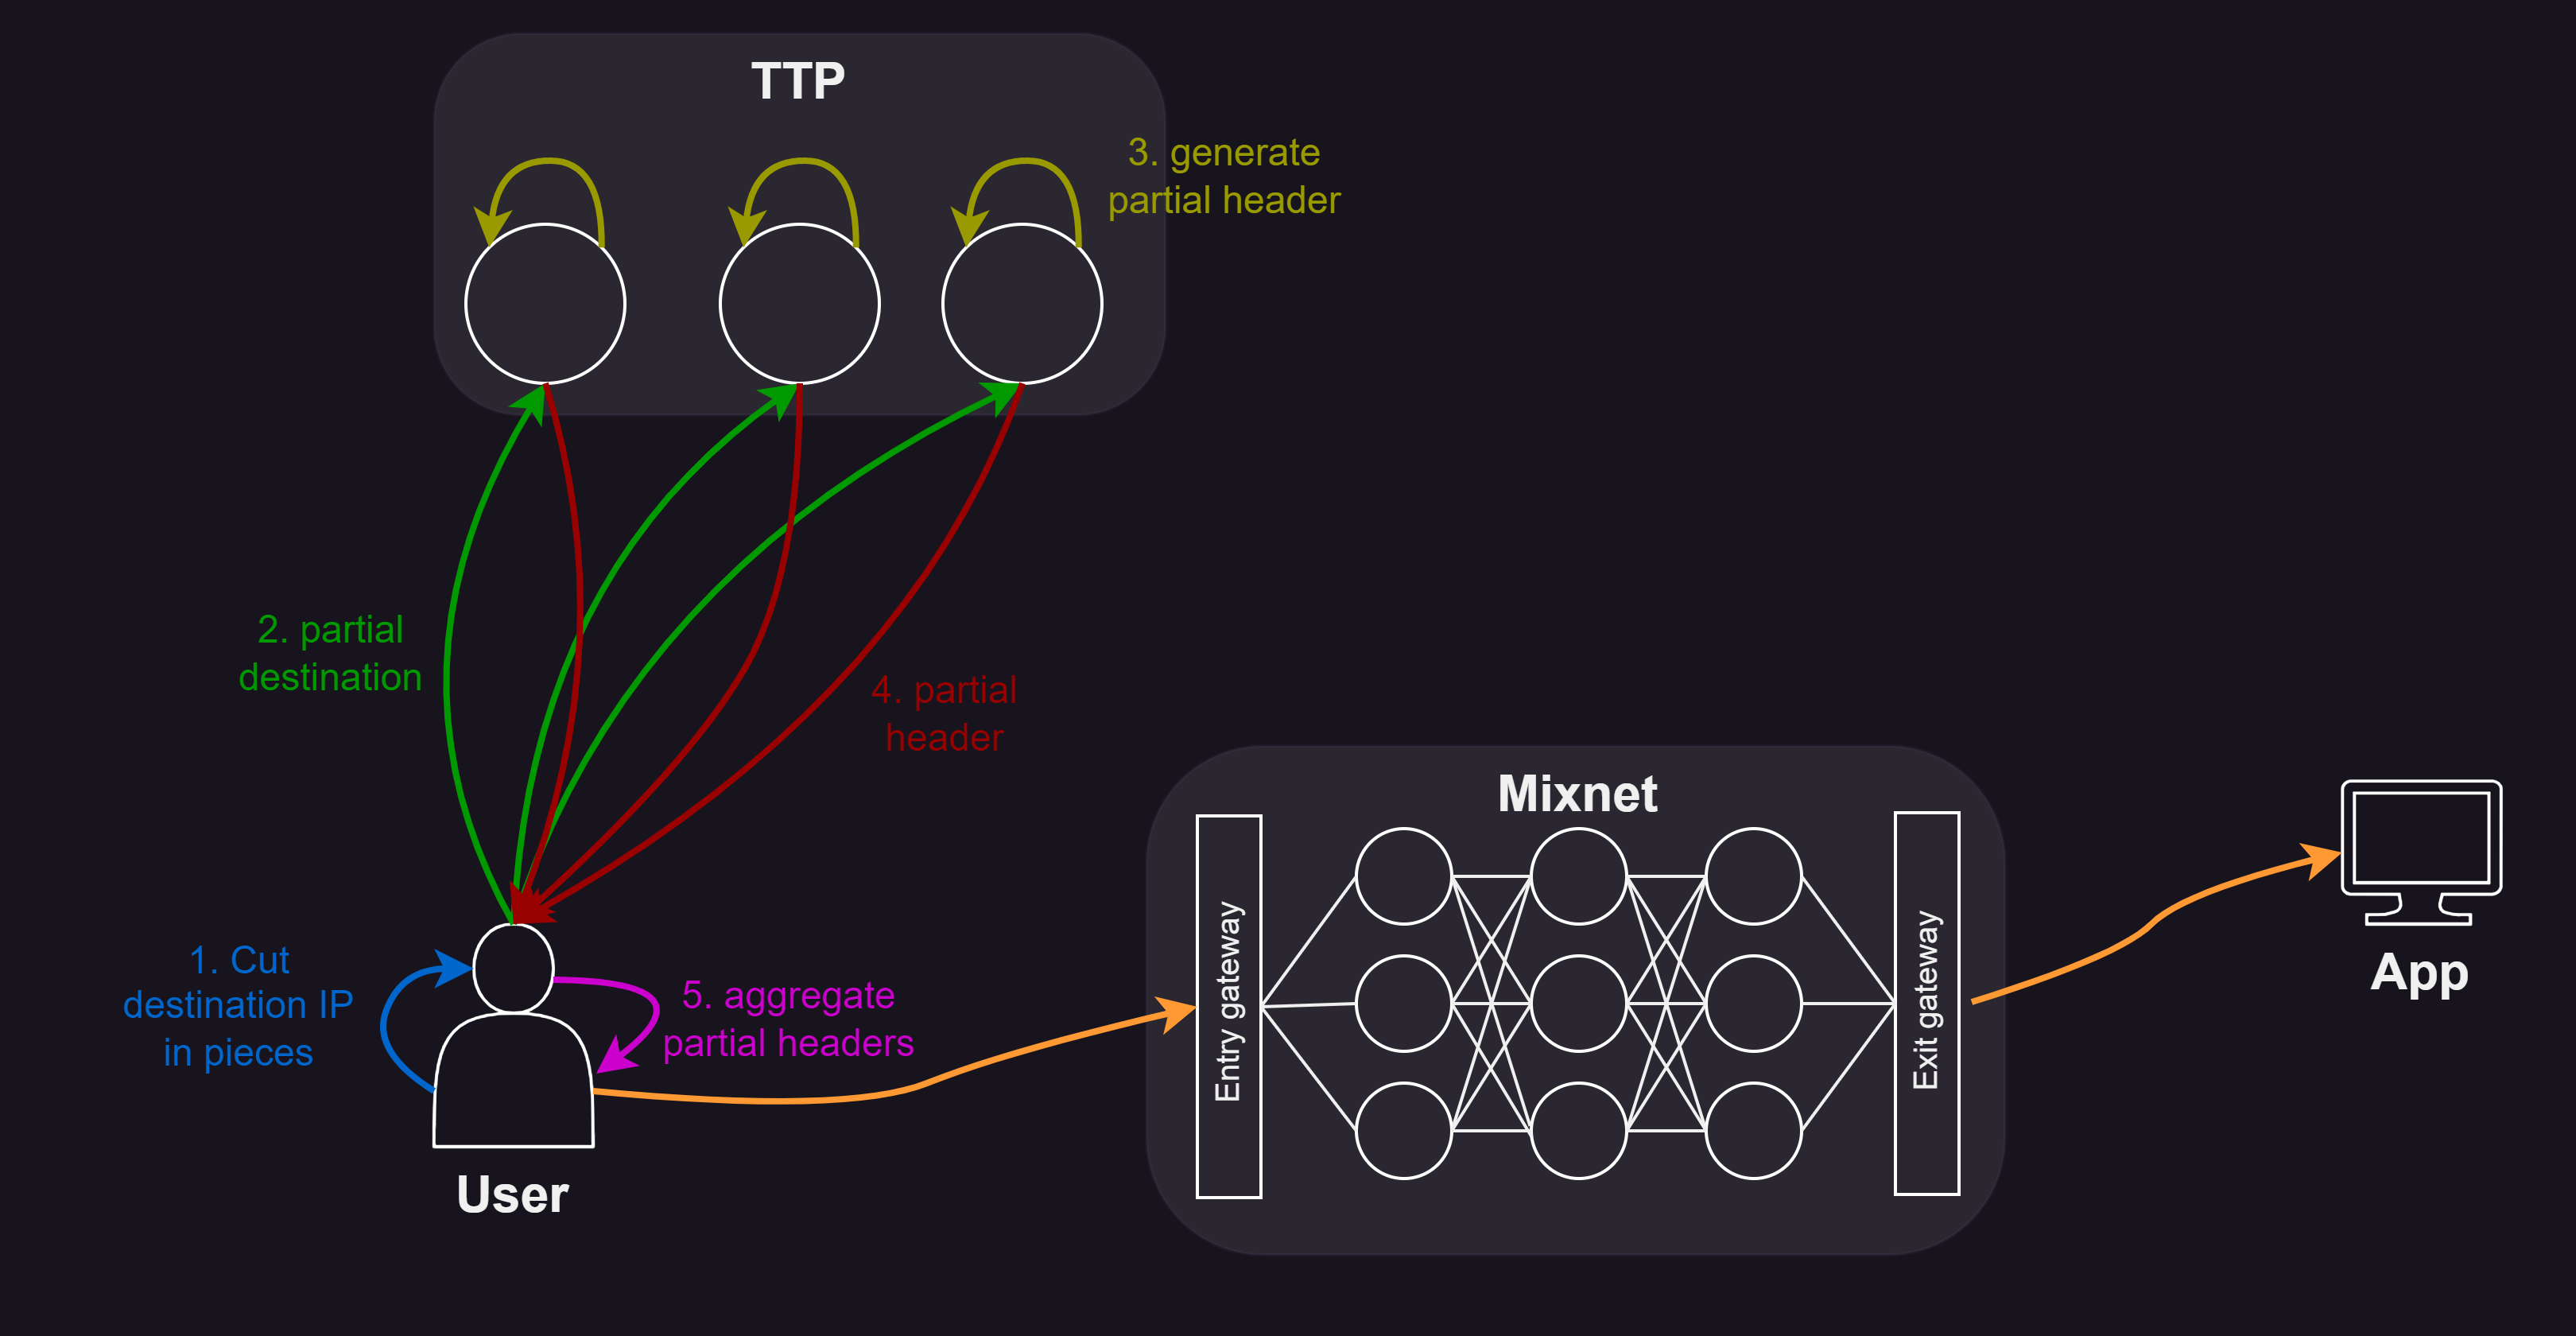
\includegraphics[width=0.5\linewidth]{Images/sphinx_ttp.png}
    \caption{Overview of the decentralized scheme\todo{Iness: Is there a reason why the arrows have different colors? If not than change to all black, Change "App" with "Service provider", Also I prefer a white background over black}}
    \label{fig:overall_schema}
\end{figure}

%%%%%%%%%%%%%%%
%One major challenge in decentralizing the original sphinx schema (Figure \ref{fig:header_cipher}) lies in the integrity tag, which is computed as the HMAC of the header $\beta_i$ using shared secret $s_i$. 
%To ensure security, no third party should have access to $s_i$, as collusion among third parties could lead to the recovery of all $s_i$, enabling them to decrypt the header and payload.
%To address this, third parties could compute a portion of the HMAC using a fragment of the shared secret $s_i$, and then combine these partial HMACs to produce the final HMAC. 
%This approach would require a hash function with homomorphic properties, which inherently weakens the collusion resistance and potentially compromises the second pre-image resistance of a secure hash.
%%%%%%%%%%%%%%%

\todo{I'd rather specify the requirements for the hash here.}
The main issue with the choosen approach is that we have to compute integrity tag on partial header such 
that combining those partial integrity tag gives the integrity tag of the final header.
However, even if breaking this homomorphic hash is feasible, if it remains computationally hard enough (e.g., requiring several hours), it could still be considered sufficiently secure for our purposes.
% TODO: VERIFY WHY NEED TO BE PER CHUNK
% What append if size secret bigger than chunk size (more random ?)


% ALPHA - 3 possibilities
% 1) Sending 1 alpha that is derived at each mixnode to generate a new alpha (efficient and clean but maybe not random enough)
    %  a) $\alpha_{i+1} = \alpha_i^{hash(\alpha_i, s_i)}$  -> article version
    %  b) $\alpha_{i+1} = G^{hash(\alpha_i, s_i)}$  --> Avoid "(x*b) % (mod-1)" in the exp -> less constraints
    %  c) $\alpha_{i+1} = \alpha_i^{2 s_i+1}$
    %  D) $\alpha_{i+1} = G^{\alpha_i (2 s_i+1)}$
% 2) Sending 1 alpha (unchanged) that is encrypted at each mixnode for the next one node (slower)
% 3) Sending 3 alpha (esay, robust but not size efficent) 

% BETA
% 1) compute by chunk
% 2) compute the whole ==> Possible ? If yes/no on which cases 

% GAMMA
% 0) User sends hash(s_i) if computed by layer
% 1) Using a different secret (s'_i) for integrity that is common to all TTP (for RSA) ==> i.e. different message, same secret
        % Pro: Easier
        % Con: Need an extra secret to send and key to handle
% 2̶)̶ ̶U̶s̶i̶n̶g̶ ̶p̶a̶r̶t̶i̶a̶l̶ ̶s̶_̶i̶ ̶o̶n̶ ̶p̶a̶r̶t̶i̶a̶l̶ ̶b̶e̶t̶a̶_̶i̶ ̶=̶=̶>̶ ̶i̶.̶e̶.̶ ̶d̶i̶f̶f̶e̶r̶e̶n̶t̶ ̶m̶e̶s̶s̶a̶g̶e̶,̶ ̶d̶i̶f̶f̶e̶r̶e̶n̶t̶ ̶s̶e̶c̶r̶e̶t̶
        %̶ ̶e̶.̶g̶.̶ ̶(̶s̶_̶i̶1̶ ̶*̶ ̶b̶'̶_̶i̶1̶)̶ ̶*̶ ̶(̶s̶_̶i̶2̶ ̶*̶ ̶b̶'̶_̶i̶2̶)̶ ̶*̶ ̶(̶.̶.̶.̶)̶ ̶=̶=̶>̶ ̶b̶'̶ ̶m̶u̶s̶t̶ ̶b̶e̶ ̶t̶h̶e̶ ̶f̶r̶e̶s̶h̶ ̶c̶o̶m̶p̶u̶t̶e̶d̶ ̶b̶ ̶(̶n̶o̶t̶ ̶t̶h̶e̶ ̶p̶r̶e̶v̶i̶o̶u̶s̶ ̶o̶n̶e̶)̶
        % /!\ LEAK INFORMATION (about s_i) /!\
